
\newcommand{\Traj}{\mathcal T}
\DeclareDocumentCommand{\Stab}{s}{\mathcal{S}\IfBooleanT{#1}{\vert_{\W_y=0}}}
\newcommand{\Fail}{\mathcal F}
\DeclareDocumentCommand{\g}{s}{\gamma\IfBooleanT{#1}{_{eff}}}
\newcommand{\CO}{\mathrm{CO}}
\renewcommand{\D}{\mathcal D}

\subsection{Calibration algorithm}
Let $\Traj$ denote the set of all trajectories that a particle might follow in the accelerator.
$\Traj = \Stab \bigcup \Fail$, where $\Stab$ is the set of all stable trajectories, $\Fail$ are all trajectories
such that if a particle gets on one, it will be lost from the bunch.

Calibration is done in two phases:
\begin{enumerate}
\item In the first phase, the guide field value is set so that the beam particles are injected onto trajectories
  $t\in\Stab$.
\item In the second phase, it is fine-tuned further, so as to fulfill the FS condition in the horizontal plane.
  By doing this, we physically move the beam trajectories into the subset $\Stab*\subset\Stab$ of trajectories 
  for which $\w_y = 0$.
\end{enumerate}

Spin tune (and hence precession frequency) is an injective function of the
effective Lorentz-factor $\g*$, which means
$\w_y(\g*^1) = \w_y(\g*^2) \rightarrow \g*^1 = \g*^2$. The trajectory space $\Traj$ is partitioned into equivalence
classes according to the value of $\g*$: trajectories characterized by the same $\g*$ are equivalent
in terms of their spin dynamics (possess the same spin tune and invariant spin axis direction),
and hence belong to the same equivalence class.
Since $\w_y(\g*)$ is injective, there exists a unique $\g*^0$ at which $\w_y(\g*^0)=0$:
\[
[\w_y=0] = [\g*^0] \equiv \Stab*.
\]

If the lattice didn't use sextupole fields for the suppression of decoherence,
$\Stab*$ would be a singleton set. We have shown in~\ref{chpt3:decoherence} that if sextupoles are
utilized, then $\exists\D\subset\Stab$ such that $\forall t_1,t_2\in\D$:
$\nu_s(t_1) = \nu_s(t_2)$, $\nbar(t_1) = \nbar(t_2)$. By adjusting the guide field strength we equate
$\D=\Stab*$, and hence $\Stab*$ contains multiple trajectories.~\footnote{Strictly speaking,
  even if sextupoles are used there remains some negligible dependence of spin tune
  on the particle orbit length (linear decoherence effects, cf.~\ref{chpt3:decoherence}).
  Because of that, the equalities for $\nu_s$ and $\nbar$ are approximate, and the set $\Stab*$
  should be viewed as fuzzy:
  we will consider trajectories for which $|\w_y|<\delta$ for some small $\delta$ as belonging to $[\w_y=0]$.}

Therefore, once we ensured that the beam polarization does not precess in the horizontal plane,
all of the beam particles have $\g*^0$, equal for the CW and CCW beams.


In order to confirm that the proposed calibration procedure works, we need to show that:
\begin{enumerate}
\item $\Stab*^{CW} = \Stab*^{CCW}$, that is $\W_y=0$ for the same set of trajectories (equivalently,
  the same $\g*$) in the CW and CCW cases.
\item $\forall t_1,t_2\in\Stab*^{CCW}$: $\nu_s(t_1) = \nu_s(t_2)$, $\nbar(t_1) = \nbar(t_2)$, i.e., the same
  sextupole fields reduce decohrerence in the CW and CCW beams.
\end{enumerate}

Practically, we do this by:
\begin{enumerate}
\item computing the dependencies $\nu_s(z),~z\in\{x,y,\delta\}$ for the CW and CCW beams;
\item computing the discrepancy $\epsilon(z) = \nu_s^{CW}(z) - \nu_s^{CCW}(z)$.
\end{enumerate}

If the discrepancy is small in a wide range of $z$, then
\begin{enumerate}
\item sextupole decoherence suppression works for both beams without gradient value change;
\item spin tune (respectively $\g*$) is equal for both beams, and hence their Spin Wheels roll at the
  same rate.
\end{enumerate}

The $\nbar^{CW}$, $\nbar^{CCW}$ tilt angles relative to the closed orbit plane are determined by the accuracy of
setting $\W_y=0$.

\subsection{Simulation}
In the simulation, we use an imperfect FS lattice~\cite{Senichev:Lattices}, in which the E+B
spin rotator elements are tilted about the optic axis by angles 
\[
\alpha\sim N(0, 5\cdot 10^{-4})\text{~rad}.
\]
Spin decoherence is being suppressed. The simulation is repeated three times;
each time only one sextupole family is turned on.
Each family's sextupole gradieent is optimized according to the procedure
described in section~\ref{sec:decoh:suppression_in_ideal_lattice}.

The beam kinetic energy is 270.00 MeV. We compute third-order Taylor expansions of the
spin and orbital transfer maps.

The main body of the simulation consists in the following: using the TSS~\cite[p.~41]{COSYINF:Manual:BeamPhys}
procedure
of COSY Infinity we compute the $\nu_s$ and $\nbar$ third-order Taylor expansions for the lattice traversed
in the forward direction.
Then, using the combinations of procedures MR and SMR~\cite[p.~233]{Eremey:Thesis}, we reverse
the lattice's orbital and spin transfer maps, and compute $\nu_s$ and $\nbar$
for the reversed lattice (as it is seen by the counter-circulating beam).


\subsection{Results}

The test results are shown in Figures~\ref{fig:X:calib_plot}, \ref{fig:Y:calib_plot}, and~\ref{fig:D:calib_plot}. Specifically, in Figures~\ref{fig:X:calib_plot:stune},
\ref{fig:Y:calib_plot:stune}, and~\ref{fig:D:calib_plot:stune} we plotted CW and CCW beams' $\nu_s$ and $\nbar_y$
as functions of the particle's transverse ($x$, $y$) and energy ($\delta$) phase space coordinates,
 respectively. One can see that the $\nu_s^{CW}$ and $\nu_s^{CCW}$ dependencies (as well as
$\nbar_y^{CW}$ and $\nbar_y^{CCW}$) differ, but at the same time the beams' $\Delta\W_y$ discrepancy does not
exceed $\pm3\cdot10^{-6}$~rad/sec; the spin tune discrepancy is below $10^{-13}$, that of the transverse
components of $\nbar$ the $10^{-8}$ level. Figures~\ref{fig:X:calib_plot:omegas}, \ref{fig:Y:calib_plot:omegas},
and~\ref{fig:D:calib_plot:omegas} show the difference between the CW \& CCW beams' spin precession
angular velociy vectors' radial components as a function of their vertical component difference. 
One can observe,
that when the difference $\Delta\W_y < 10^{-7}$ rad/sec (this is the statistical precision
of a frequency estimate achievable in one cycle), the difference $\Delta \W_x < 10^{-8}$~rad/sec (i.e.,
an order of magnitude less than the statistical precision).
This confirmes that the equalization of the vertical plane MDM precession frequencies of counter-circulating
beams by means of equalizing their horizontal plane precession frequencies is a viable technique.

\begin{figure}[h]
  \centering
  \begin{subfigure}{\linewidth}
    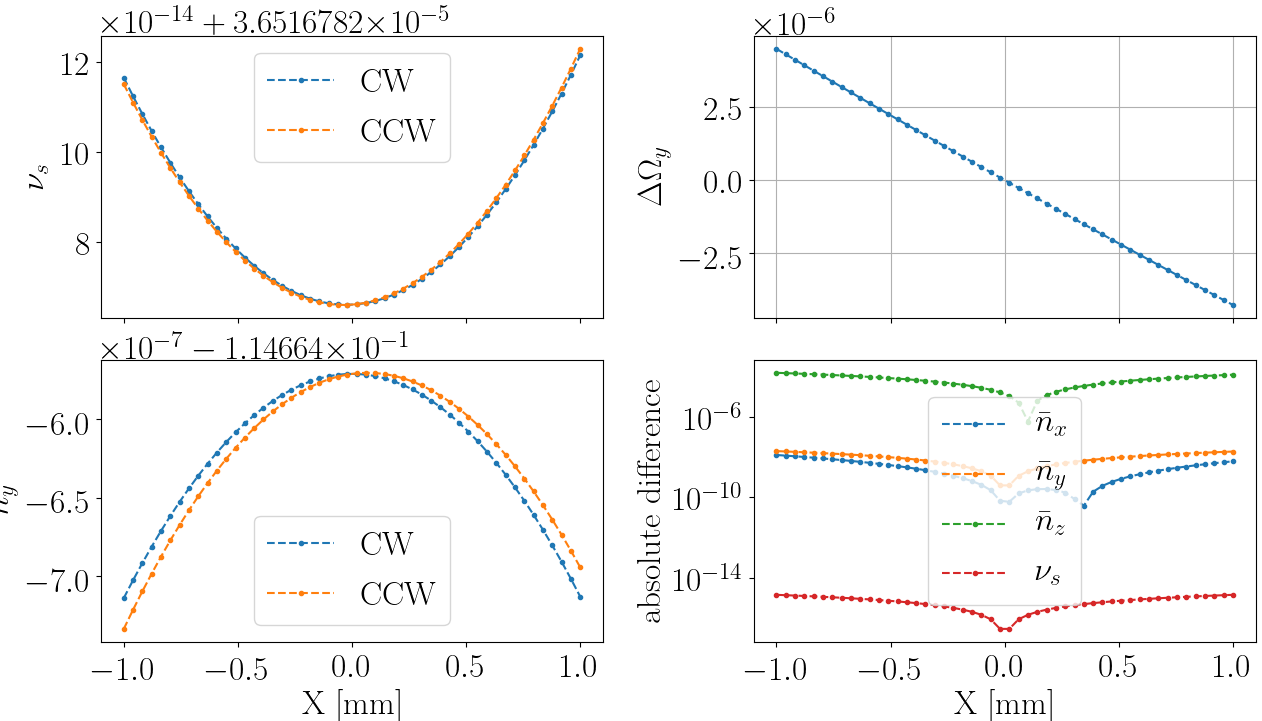
\includegraphics[width=\linewidth]{images/GFF/GFF_stune_range_X}
    \caption{Spin tune and invariant spin axis as functions of the particle's
      horizontal offset from the closed orbit.\label{fig:X:calib_plot:stune}}
  \end{subfigure}
  \begin{subfigure}{\linewidth}
    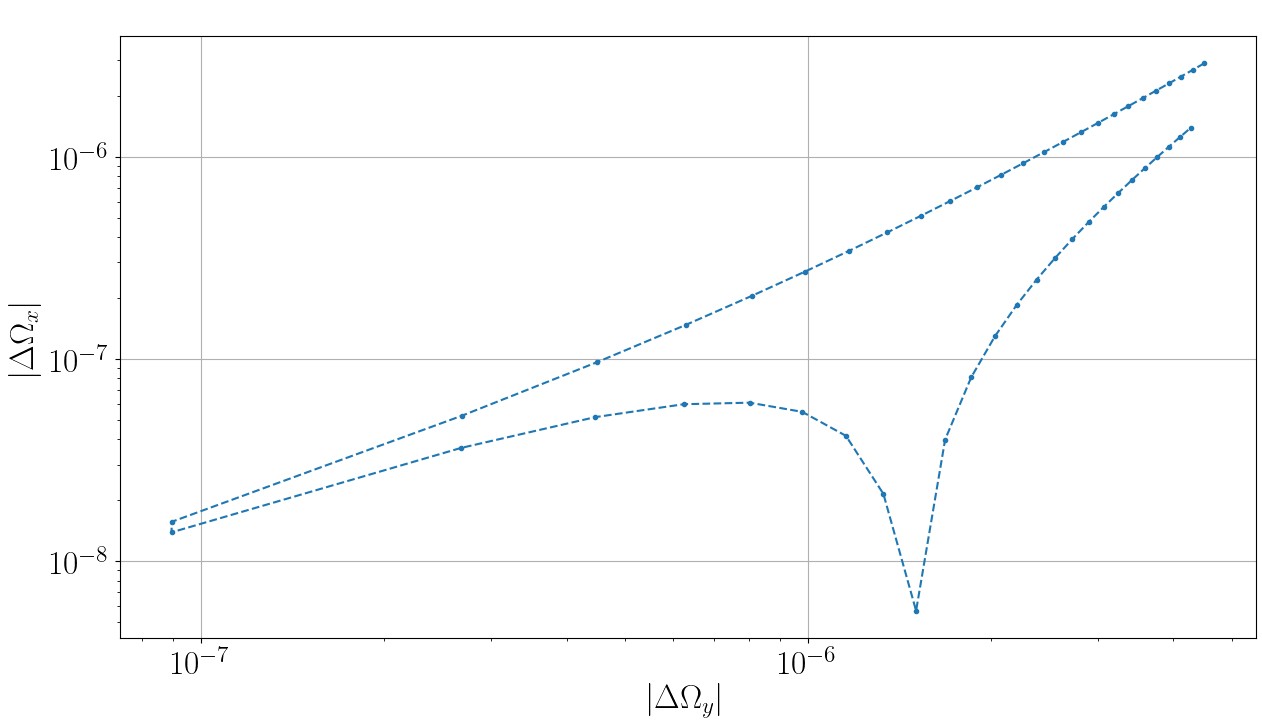
\includegraphics[width=\linewidth]{images/GFF/GFF_omegas_range_X}
    \caption{Difference between the CW \& CCW beams' radial spin precession angular velocity components
      as a function of the differnce between their vertical components
      (calibration plot).\label{fig:X:calib_plot:omegas}}
  \end{subfigure}    
  \caption{Simulation results in the case fo horizontal plane betatron motion-related
    spin decoherence.\label{fig:X:calib_plot}}
\end{figure}

\begin{figure}[h]
  \centering
  \begin{subfigure}{\linewidth}
    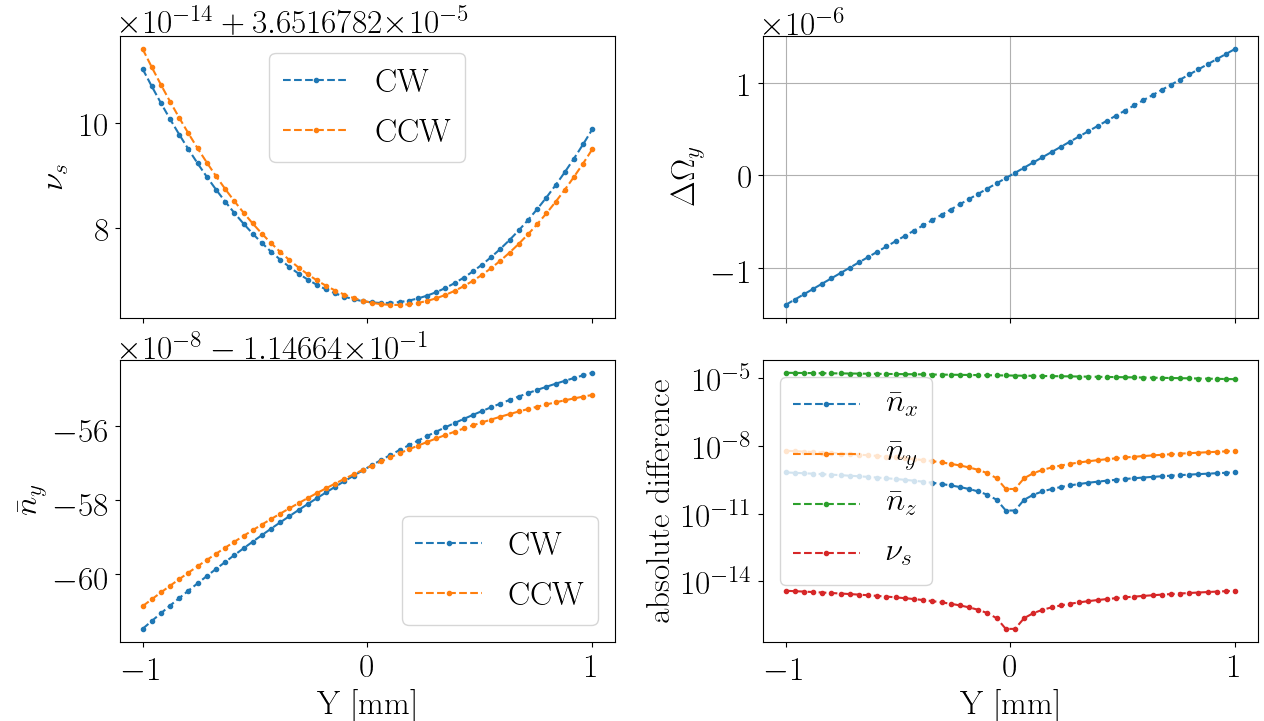
\includegraphics[width=\linewidth]{images/GFF/GFF_stune_range_Y}
    \caption{Spin tune and invariant spin axis as functions of the particle's
      vertical offset from the closed orbit.\label{fig:Y:calib_plot:stune}}
  \end{subfigure}
  \begin{subfigure}{\linewidth}
    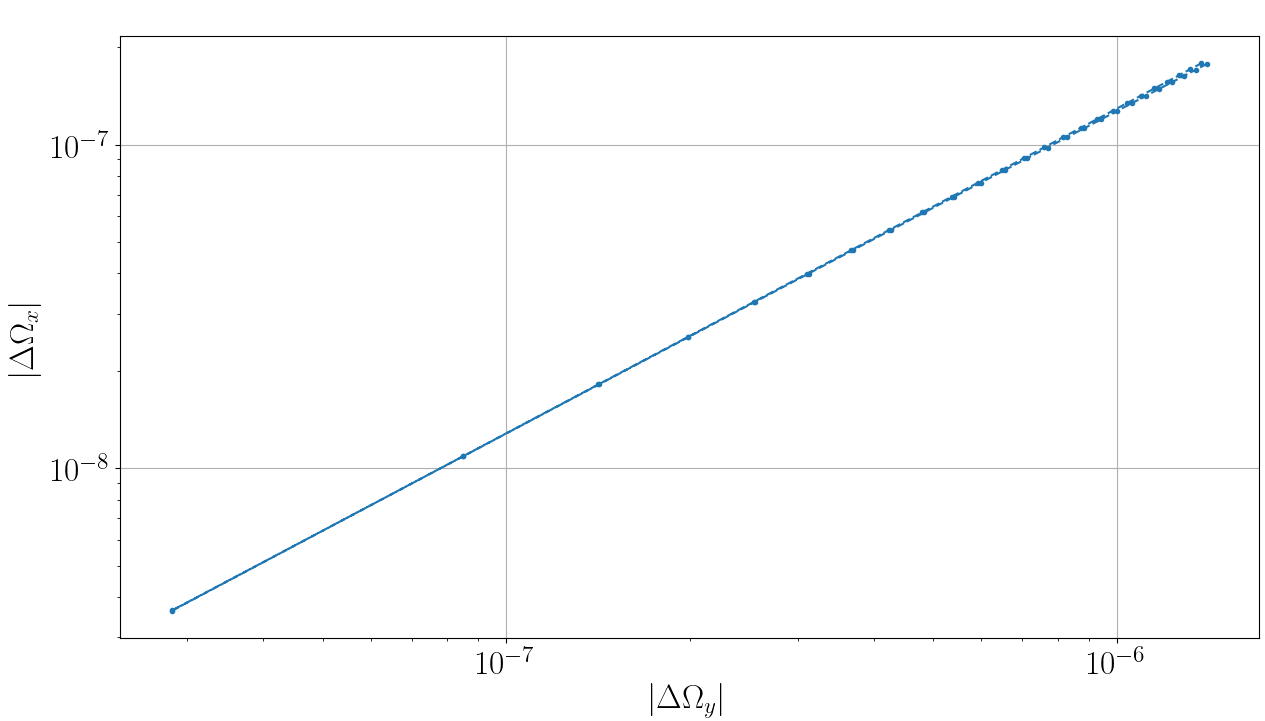
\includegraphics[width=\linewidth]{images/GFF/GFF_omegas_range_Y}
    \caption{Difference between the CW \& CCW beams' radial spin precession angular velocity components
      as a function of the differnce between their vertical components
      (calibration plot).\label{fig:Y:calib_plot:omegas}}
  \end{subfigure}    
  \caption{Simulation results in the case fo vertical plane betatron motion-related
    spin decoherence.\label{fig:Y:calib_plot}}
\end{figure}

\begin{figure}[h]
  \centering
  \begin{subfigure}{\linewidth}
    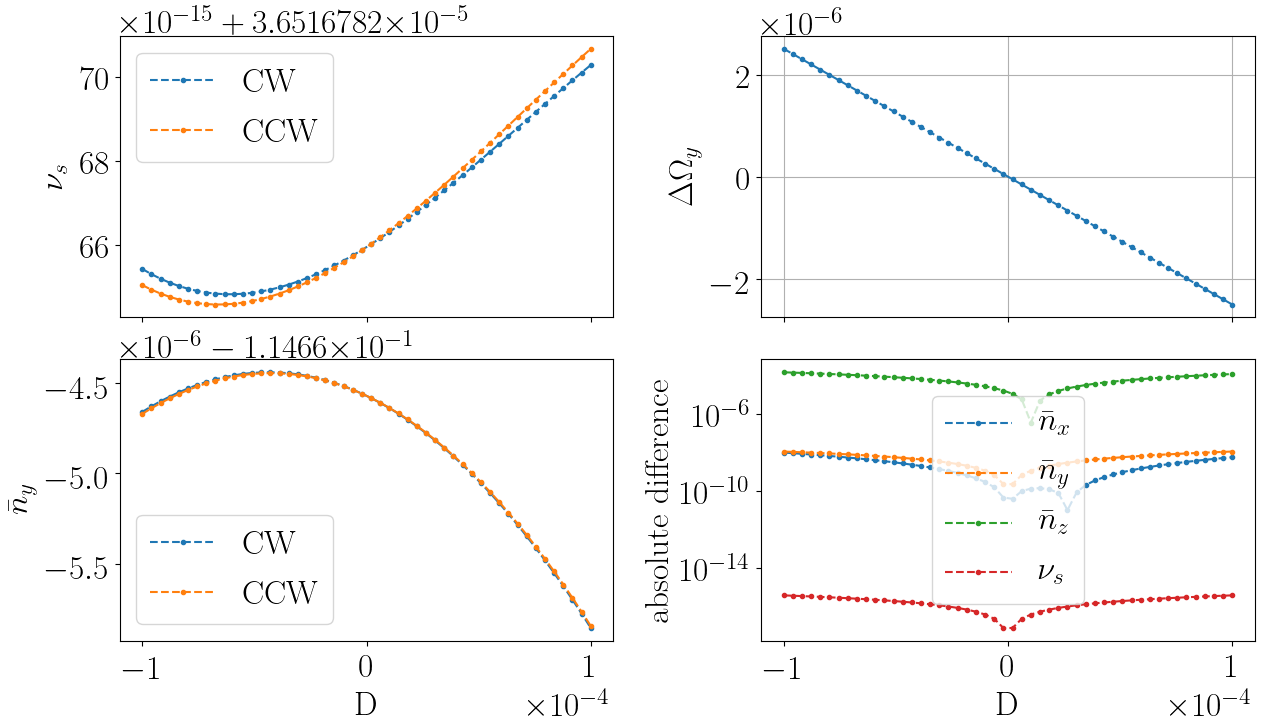
\includegraphics[width=\linewidth]{images/GFF/GFF_stune_range_D}
    \caption{Spin tune and invariant spin axis as functions of the particle's
      energy offset from the reference energy.\label{fig:D:calib_plot:stune}}
  \end{subfigure}
  \begin{subfigure}{\linewidth}
    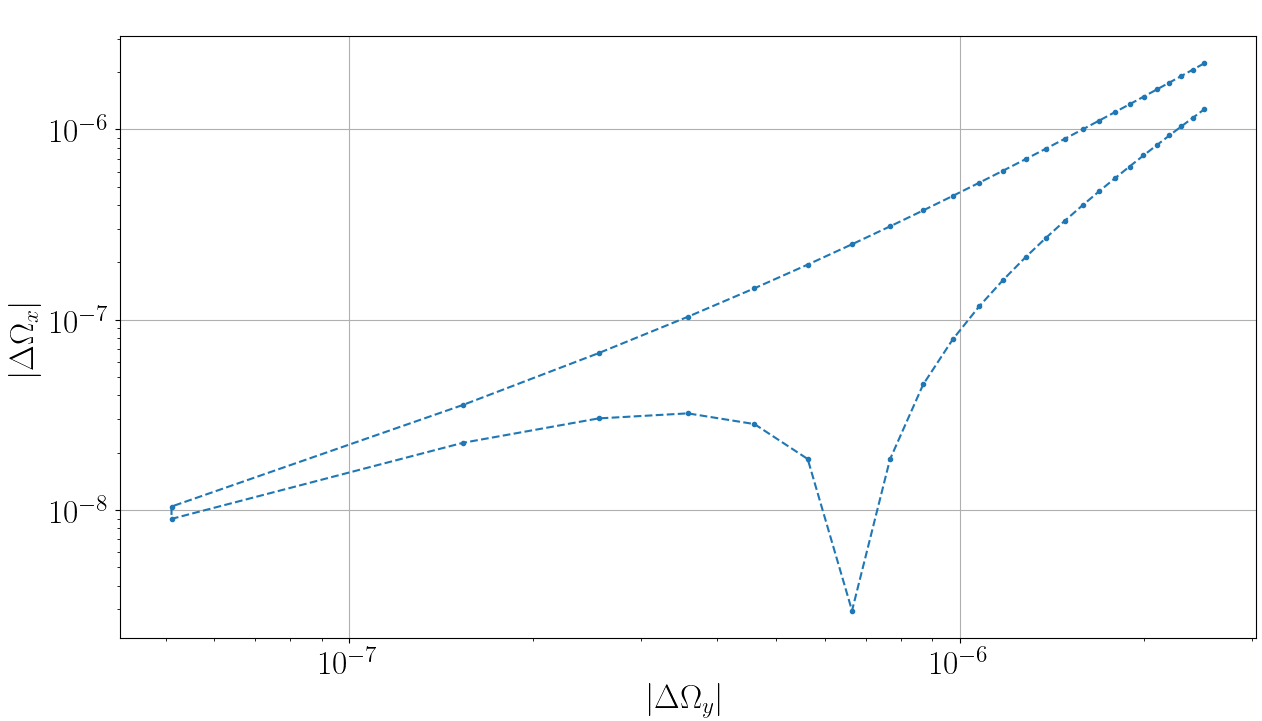
\includegraphics[width=\linewidth]{images/GFF/GFF_omegas_range_D}
    \caption{Difference between the CW \& CCW beams' radial spin precession angular velocity components
      as a function of the differnce between their vertical components
      (calibration plot).\label{fig:D:calib_plot:omegas}}
  \end{subfigure}    
  \caption{Simulation results in the case fo vertical plane synchrotron oscillations-related
    spin decoherence.\label{fig:D:calib_plot}}
\end{figure}
